\section{Sändare}
\label{sändare}
\index{sändare}

\subsection{Blockschema}
\index{blockschema}

\emph{Blockschema} är sätt att göra en översiktlig principskiss över en
apparats design, där de övergripande principerna för funktionen är illustrerade
i en förenklad form där varje block representerar en grundläggande funktion.
Denna förenkling gör att man kan snabb få en översikt utan att fastna i
konstruktionsdetaljerna av enstaka block.

Hela apparaten kan ses som ett antal funktionsblock. Hur de samverkar
framgår i stort av blockschemat.
Där återfinns oscillatorer, blandare, förstärkare etc.
I schemat kan även finnas uppgifter om frekvenser och spänningar m.m.

Det finns olika slags funktionsblock -- kretsar. Kombinationen av block
ger apparater med olika egenskaper.
Exempel är s.k. raka sändare med samma frekvens genom hela sändaren,
superheterodynsändare där frekvensblandning används,
frekvensmultiplicerande sändare etc.

\subsection{Rak sändare}
\textbf{HAREC
  a.\ref{HAREC.a.5.1.1b}\label{myHAREC.a.5.1.1b},
  a.\ref{HAREC.a.5.2.1}\label{myHAREC.a.5.2.1},
  a.\ref{HAREC.a.5.3.3}\label{myHAREC.a.5.3.3}
}
\index{rak sändare}
\index{sändare!rak}

\begin{wrapfigure}{R}{0.5\textwidth}
  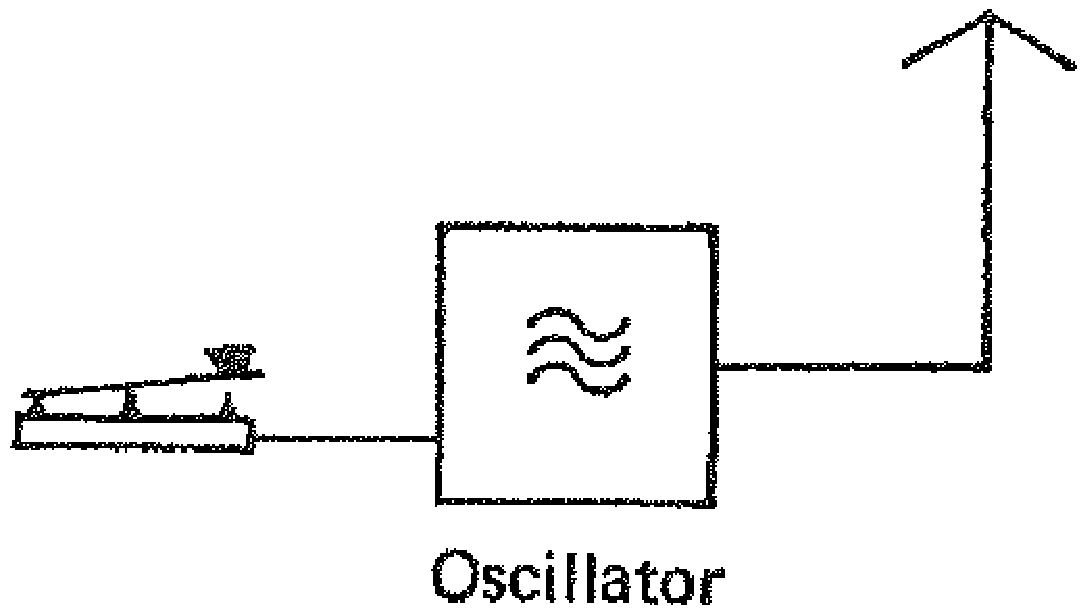
\includegraphics[width=0.5\textwidth]{images/cropped_pdfs/bild_2_5-01.pdf}
  \caption{Enstegs sändare}
  \label{fig:bildII5-1}
\end{wrapfigure}

En \emph{rak sändare}, som illustreras i bild \ref{fig:bildII5-1}, är det
enklaste sändarkonceptet.
Då är oscillatorns frekvens samma som sändningsfrekvensen och ingen
frekvensomvandling sker i signalvägen.
Om en antenn kopplas till oscillatorn så blir den en enkel enstegs sändare.

I flerstegs raka sändare följs oscillatorn av ytterligare funktioner
på samma frekvens som oscillatorn.
Buffertsteg, drivsteg och slutsteg kan vara sådana funktioner.

\begin{figure}
  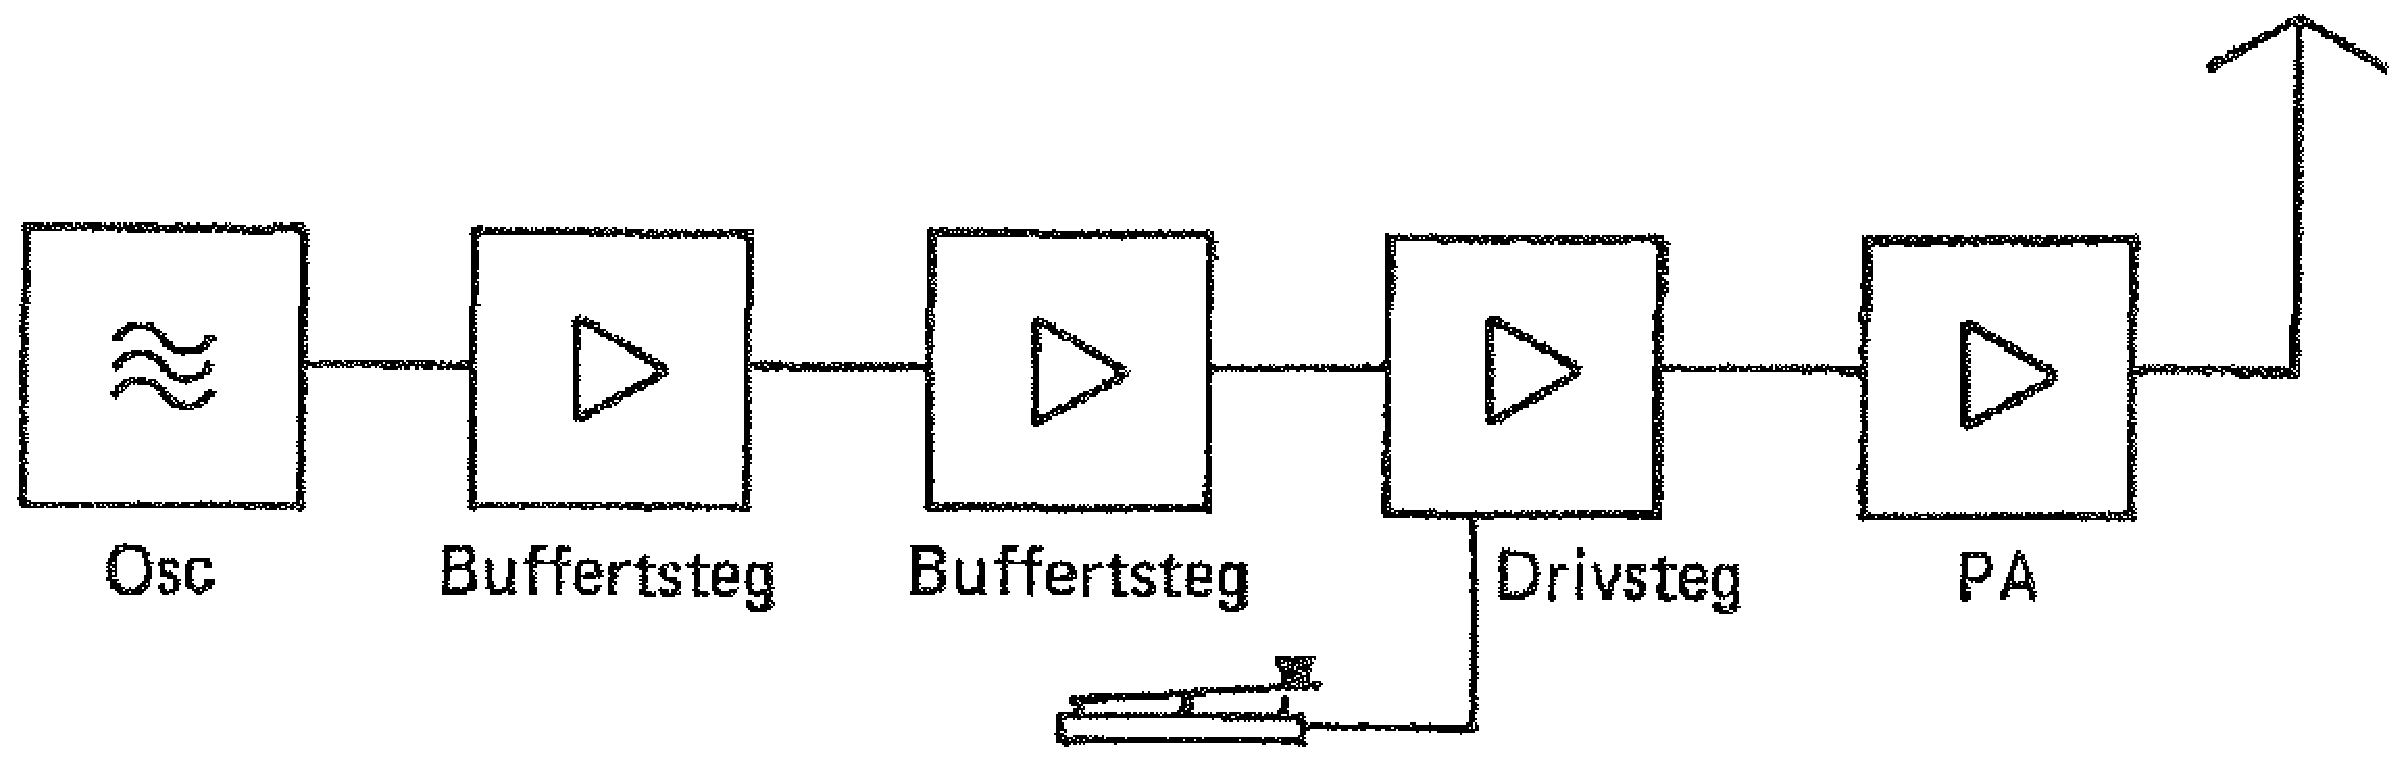
\includegraphics[width=\textwidth]{images/cropped_pdfs/bild_2_5-02.pdf}
  \caption{Flerstegs rak sändare}
  \label{fig:bildII5-2}
\end{figure}

Bild \ref{fig:bildII5-2} visar en rak sändare, som består av oscillator +
buffertsteg 1 + buffertsteg 2 + drivsteg + effektförstärkare.

Oscillatorn följs av ett avlastande buffertsteg 1.
På så sätt blir oscillatorns frekvensstabilitet bättre.
Buffertsteg 2 avlastar ytterligare och matar dessutom ett effekthöjande
drivsteg, som ger driveffekt till slutsteget, samt slutsteget där den slutliga
effekthöjningen sker.

Raka sändare kan användas för CW, FM, PM och AM, men inte DSB och SSB.
Fördelen med raka sändare är enkelheten.
Nackdelen är att alla steg arbetar på samma frekvens, varvid risken för
återverkan på ett föregående funktionssteg är större.
Oönskad återkoppling kan då bli följden, som kan ge ostabila egenskaper hos
sändaren.
Genom att i första hand bygga in VFO och buffertstegen i metallkapslingar,
s.k. skärmar, så minskas denna risk då högre isolation åstadkoms.

\subsection{Sändare med frekvensmultiplicering}
\textbf{HAREC
 a.\ref{HAREC.a.5.3.2}\label{myHAREC.a.5.3.2},
 a.\ref{HAREC.a.5.3.5}\label{myHAREC.a.5.3.5},
 a.\ref{HAREC.a.5.3.6}\label{myHAREC.a.5.3.6},
 a.\ref{HAREC.a.5.3.8}\label{myHAREC.a.5.3.8},
 a.\ref{HAREC.a.5.3.9}\label{myHAREC.a.5.3.9},
 a.\ref{HAREC.a.5.3.11}\label{myHAREC.a.5.3.11}
}
\index{frekvensmultiplicering}
\index{sändare!frekvensmultiplicering}
\index{utgångsfilter}
\index{sändare!utgångsfilter}

Helst väljer man en arbetsfrekvens för oscillatorn där den är mest
frekvensstabil.

Om högre frekvens önskas på nyttosignalen, så kan man
t.ex. multiplicera oscillatorfrekvensen, detta kallas för
\emph{frekvensmultiplicering} (eng. \emph{frequency multiplication}).
I olinjära kretsar alstras övertoner, som ofta utnyttjas i detta syfte.

Endast när kravet på frekvensstabilitet är lågt används den frekvens,
som VFO eller CO arbetar på, även för nyttosignalen.

\begin{figure}
  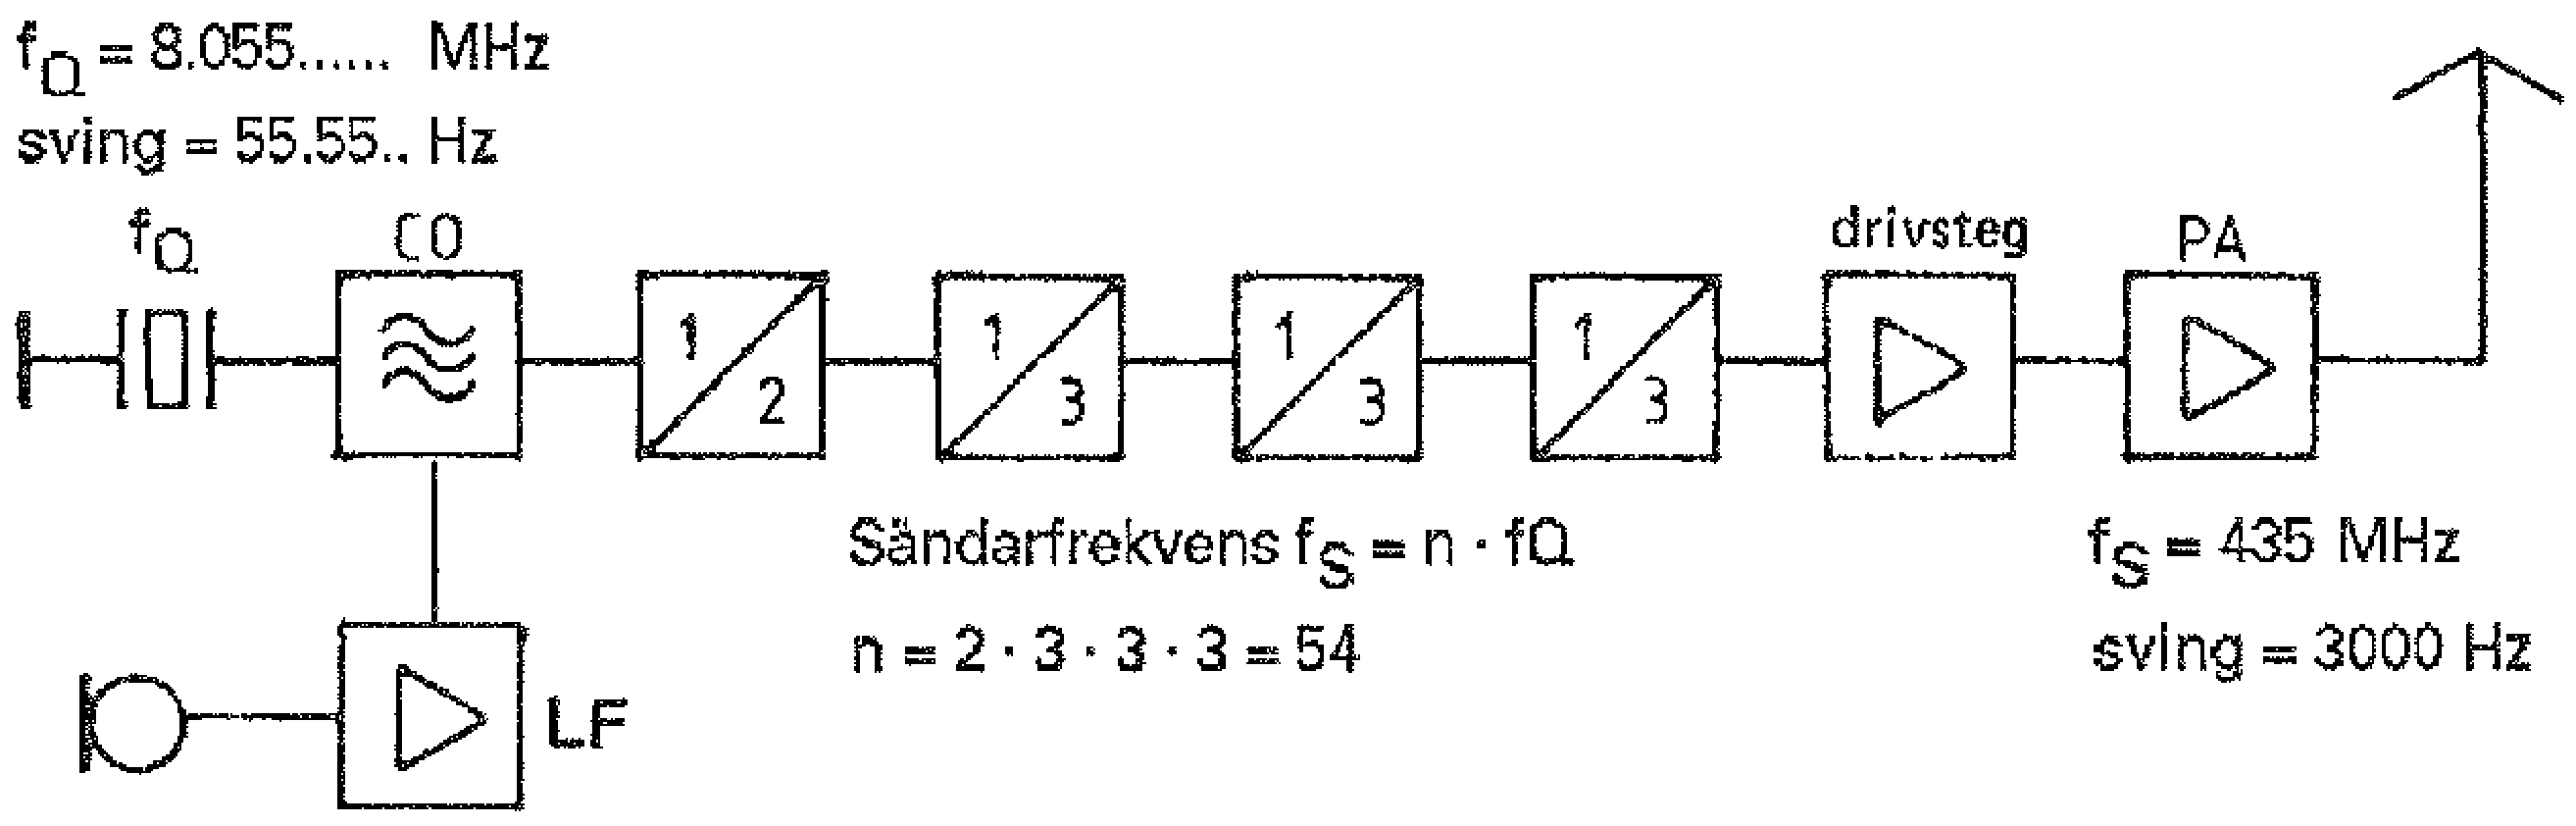
\includegraphics[width=\textwidth]{images/cropped_pdfs/bild_2_5-03.pdf}
  \caption{FM-sändare med frekvensmultiplicering}
  \label{fig:bildII5-3}
\end{figure}

Oscillatorn svänger här på en låg frekvens, som multipliceras i
olinjära förstärkarsteg till en hög sändningsfrekvens.
Oftast multipliceras frekvensen två eller tre gånger i vart och ett av
förstärkarstegen.

Bild \ref{fig:bildII5-3} visar ett blockschema för en FM sändare för
435~MHz (70~cm-bandet).
Oscillatorfrekvensen är 8,056~MHz.
I fyra av de efterföljande förstärkarna multipliceras frekvensen 2, 3, 3
respektive 3~gånger, alltså totalt 54~gånger.
Sändningsfrekvensen blir då \(8,056 \cdot 54 = 435\)~MHz.

Variationer i oscillatorfrekvensen blir också multiplicerade.
I detta exempel blir sändningsfrekvensens deviation 54~gånger större än
oscillatorfrekvensens deviation.
En deviation av max 3000~Hz från den nominella sändningsfrekvensen motsvaras
av följande deviation från oscillatorfrekvensen,

\[\Delta f = \frac{3000}{54} = 55,6\text{ [Hz]}\]

FM-sändare för VHF, UHF och SHF utförs ofta med
frekvensmultiplikation.
Jämfört med en rak sändare är komponentbehovet större, men i stället ger
den låga oscillatorfrekvensen god frekvensstabilitet, vilket är en fördel.
Risken för oönskade självsvängningar är mindre i en frekvensmultiplicerande
än i en rak sändare, eftersom in och utgångsfrekvenserna i flera av stegen är
olika.

Genom att ersätta frekvensmodulatorn med en fasmodulator så kan samma
sändare även användas för fasmodulerad signal.

De frekvensmultiplicerande stegen i bild \ref{fig:bildII5-3} arbetar i klass C,
d.v.s. olinjärt, vilket medför amplituddistorsion.
Vid frekvens- och fasmodulering saknar emellertid detta betydelse, eftersom
amplituden i det fallet inte är informationsbärande.

Övertoner i nyttosignalen bör dock filtreras bort, något som sker med ett
filter på utgången, det så kallade \emph{utgångsfiltret}
(eng. \emph{output filter}).

\subsection{Sändare med frekvensblandning -- superheterodynsändare}
\textbf{HAREC a.\ref{HAREC.a.5.1.1a}\label{myHAREC.a.5.1.1a}}

\subsubsection{Telegrafisändare (CW) för kortvåg}
\index{CW}
\index{sändare!CW}

\begin{figure}
  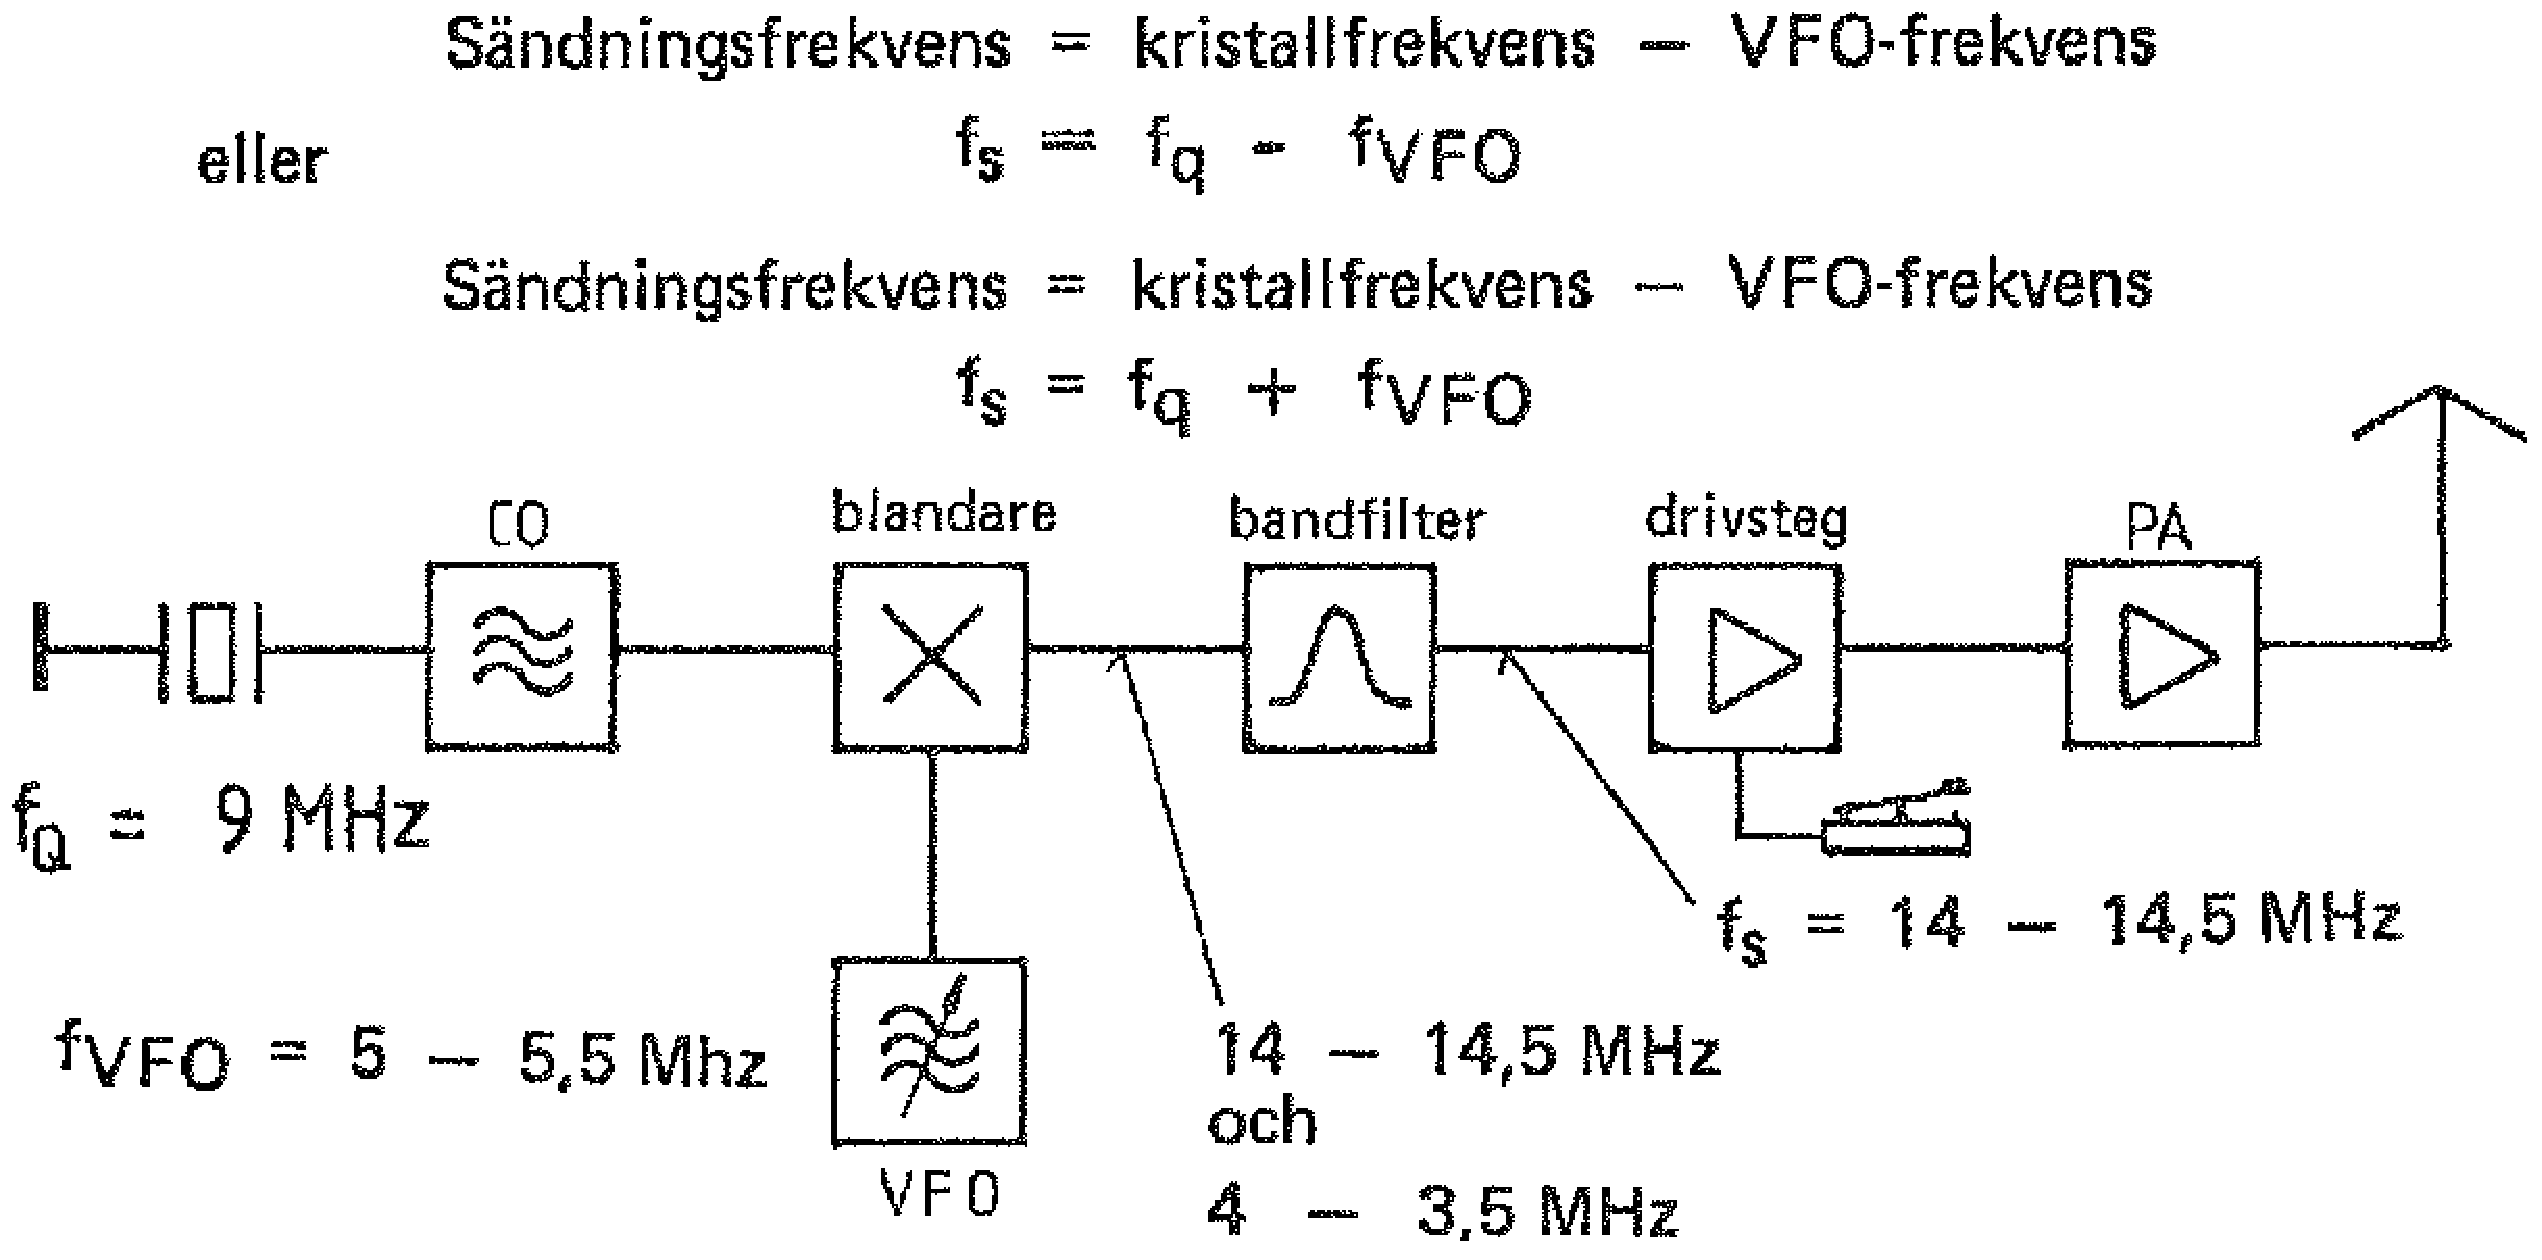
\includegraphics[width=\textwidth]{images/cropped_pdfs/bild_2_5-04.pdf}
  \caption{2-bands CW-sändare med frekvensblandning}
  \label{fig:bildII5-4}
\end{figure}

En VFO är mest stabil på låga frekvenser medan en CO har god
stabilitet även på högre frekvenser.
När signalerna från dessa blandas, bildas blandningsprodukter som är
skillnaden och summan av signalernas frekvenser.
Bild \ref{fig:bildII5-4} visar en telegrafisändare där detta fenomen används
för sändning inom området 14,0--14,5~MHz eller 3,5--4,0~MHz beroende
på passbandet i filtret efter blandaren.

Resultatet är en superheterodyn-VFO med både variabel och stabil
signal.
På bilden har valts ett filter med passband för det övre av dessa
frekvensområden.

\subsubsection{Telefonisändare (SSB) för kortvåg}
\textbf{HAREC
 a.\ref{HAREC.a.5.2.2}\label{myHAREC.a.5.2.2},
 a.\ref{HAREC.a.5.3.1}\label{myHAREC.a.5.3.1},
 a.\ref{HAREC.a.5.3.4}\label{myHAREC.a.5.3.4},
 a.\ref{HAREC.a.5.3.10}\label{myHAREC.a.5.3.10},
 a.\ref{HAREC.a.5.3.12}\label{myHAREC.a.5.3.12}
}
\index{telefoni}
\index{SSB}
\index{sändare!SSB}

\begin{figure}
  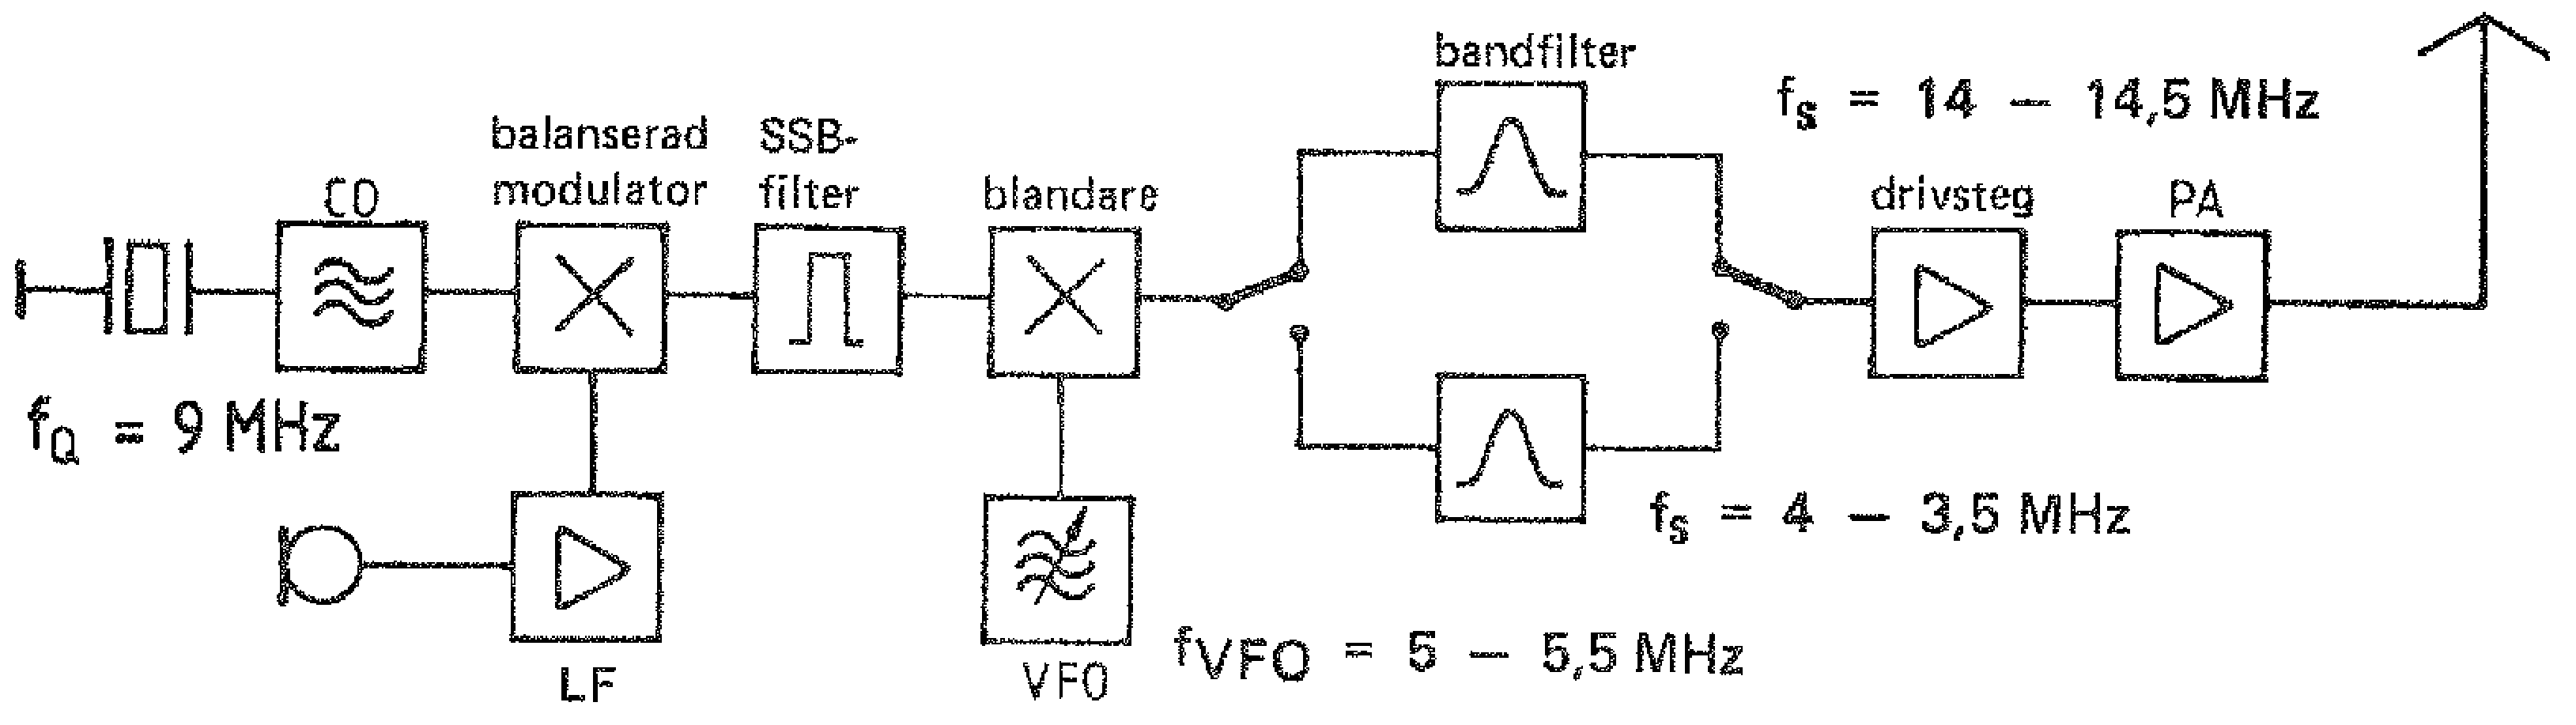
\includegraphics[width=\textwidth]{images/cropped_pdfs/bild_2_5-05.pdf}
  \caption{2-bands SSB-sändare med frekvensblandning}
  \label{fig:bildII5-5}
\end{figure}

Bild \ref{fig:bildII5-5} visar en SSB-sändare för två kortvågsband och
bygger på sändaren i bild \ref{fig:bildII5-4}.
Filtermetoden är den mest använda för att bereda en SSB-signal.
Oscillatorsignalen amplitudmoduleras i en balanserad blandare.
I en sådan undertrycks bärvågen medan de båda sidbanden släpps fram.
Det ena sidbandet undertrycks med ett bandpassfilter, ofta implementerat med
ett kristallfilter för att få god undertryckning av oönskat sidband.
Denna SSB-signal flyttas till avsett frekvensband
genom ännu en frekvensblandning och ytterligare filtrering.

I exemplet är CO-frekvensen 9~MHz. VFO har frekvensområdet 5,0--5,5~MHz.
Vid blandningen fås blandningsprodukter inom frekvensområdena
14,0--14,5~MHz och 4,0--3,5~MHz.
Genom att välja bandpassfilter kan man sända i ett av dessa frekvensområden.
Efterföljande driv- och slutsteg utförs för att arbeta i detta frekvensband,
antingen utan särskild avstämning -- s.k. bredbandigt utförande -- eller genom
avstämning på en viss frekvens, vilket ger renaste signalen.

Bild \ref{fig:bildII5-6} visar en SSB-sändare som liknar den i
bild \ref{fig:bildII5-5}.
Den stora skillnaden är att signalfrekvensen kan flyttas till flera olika band
med hjälp av ännu en frekvensblandning.
Därför används fler valbara bandpassfilter.

\begin{figure}
  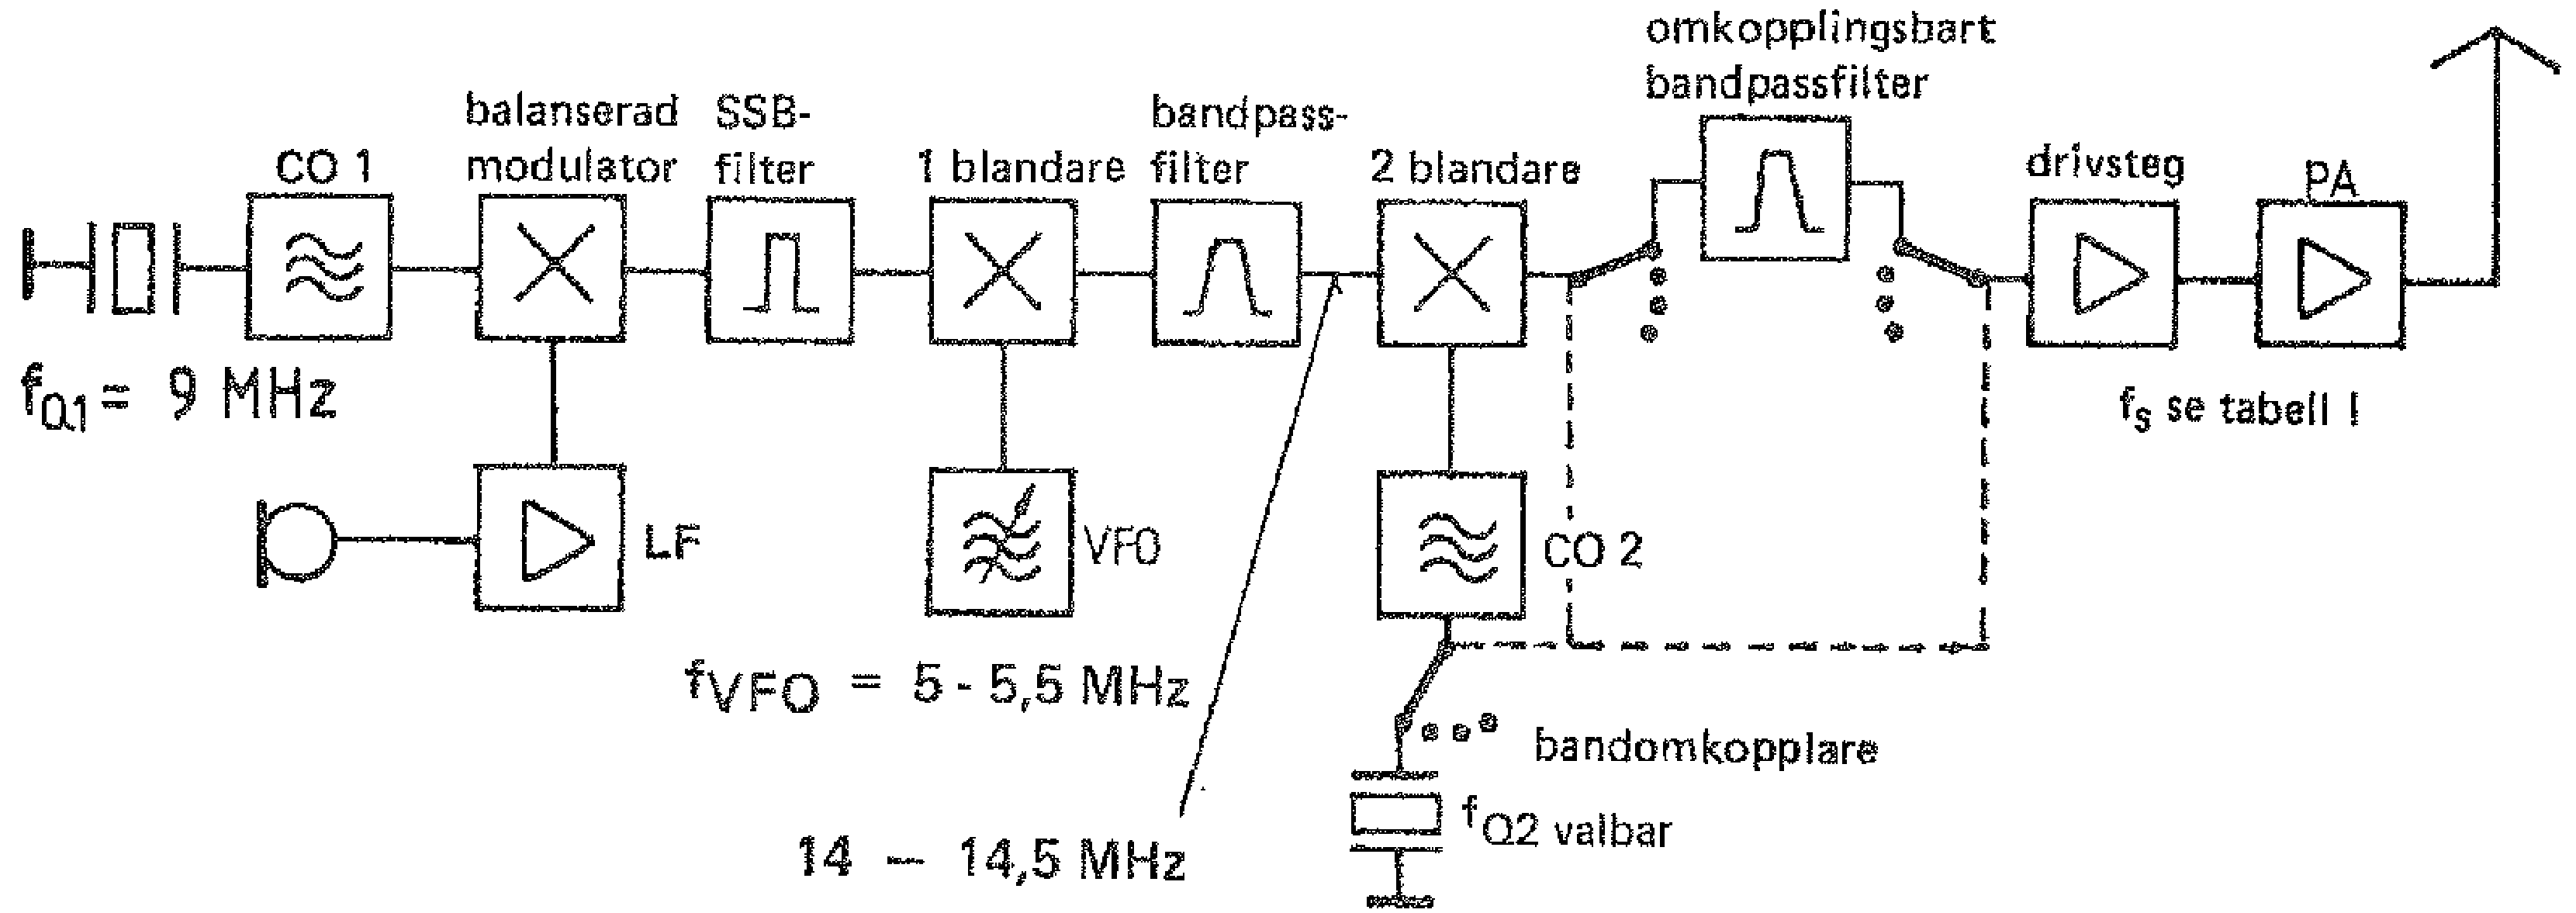
\includegraphics[width=\textwidth]{images/cropped_pdfs/bild_2_5-06.pdf}
  \caption{Flerbands SSB-sändare med frekvensblandning}
  \label{fig:bildII5-6}
\end{figure}

I en SSB-signal ligger all information i amplituden, till skillnad
från en FM-signal där all information ligger i frekvensen.
En SSB-signal får alltså inte förvrängas.
Det innebär att förstärkarstegen i SSB-sändare måste arbeta linjärt, d.v.s. en
utsignal ska vara proportionell till insignalen i varje moment.

\subsection{PLL-styrda sändare}
\index{faslåstloop}
\index{phase locked loop (PLL)}
\index{PLL}
\index{sändare!PLL}

PLL-styrning är inte ett sändarkoncept. Det är ett sätt att styra
frekvensen i en oscillator och hålla den stabil med hjälp av en
likspänning från en \emph{faslåst loop} (eng. \emph{Phase Locked Loop (PLL)})
vilket är en digitalt styrd krets.

En PLL kan användas t.ex. i raka sändare och heterodynsändare.
I det första fallet (bild \ref{fig:bildII5-2}) kan frekvensen i den enda
oscillatorn styras av en PLL.
I det andra fallet (bild \ref{fig:bildII5-6}) kan frekvensen i
någon av oscillatorerna styras av en PLL.
En närmare beskrivning av PLL-styrning av dessa två sändarkoncept följer här.

\subsubsection{PLL-styrd FM-sändare för 144--146~MHz}
\textbf{HAREC
  a.\ref{HAREC.a.5.2.3}\label{myHAREC.a.5.2.3}
}

\begin{figure}
  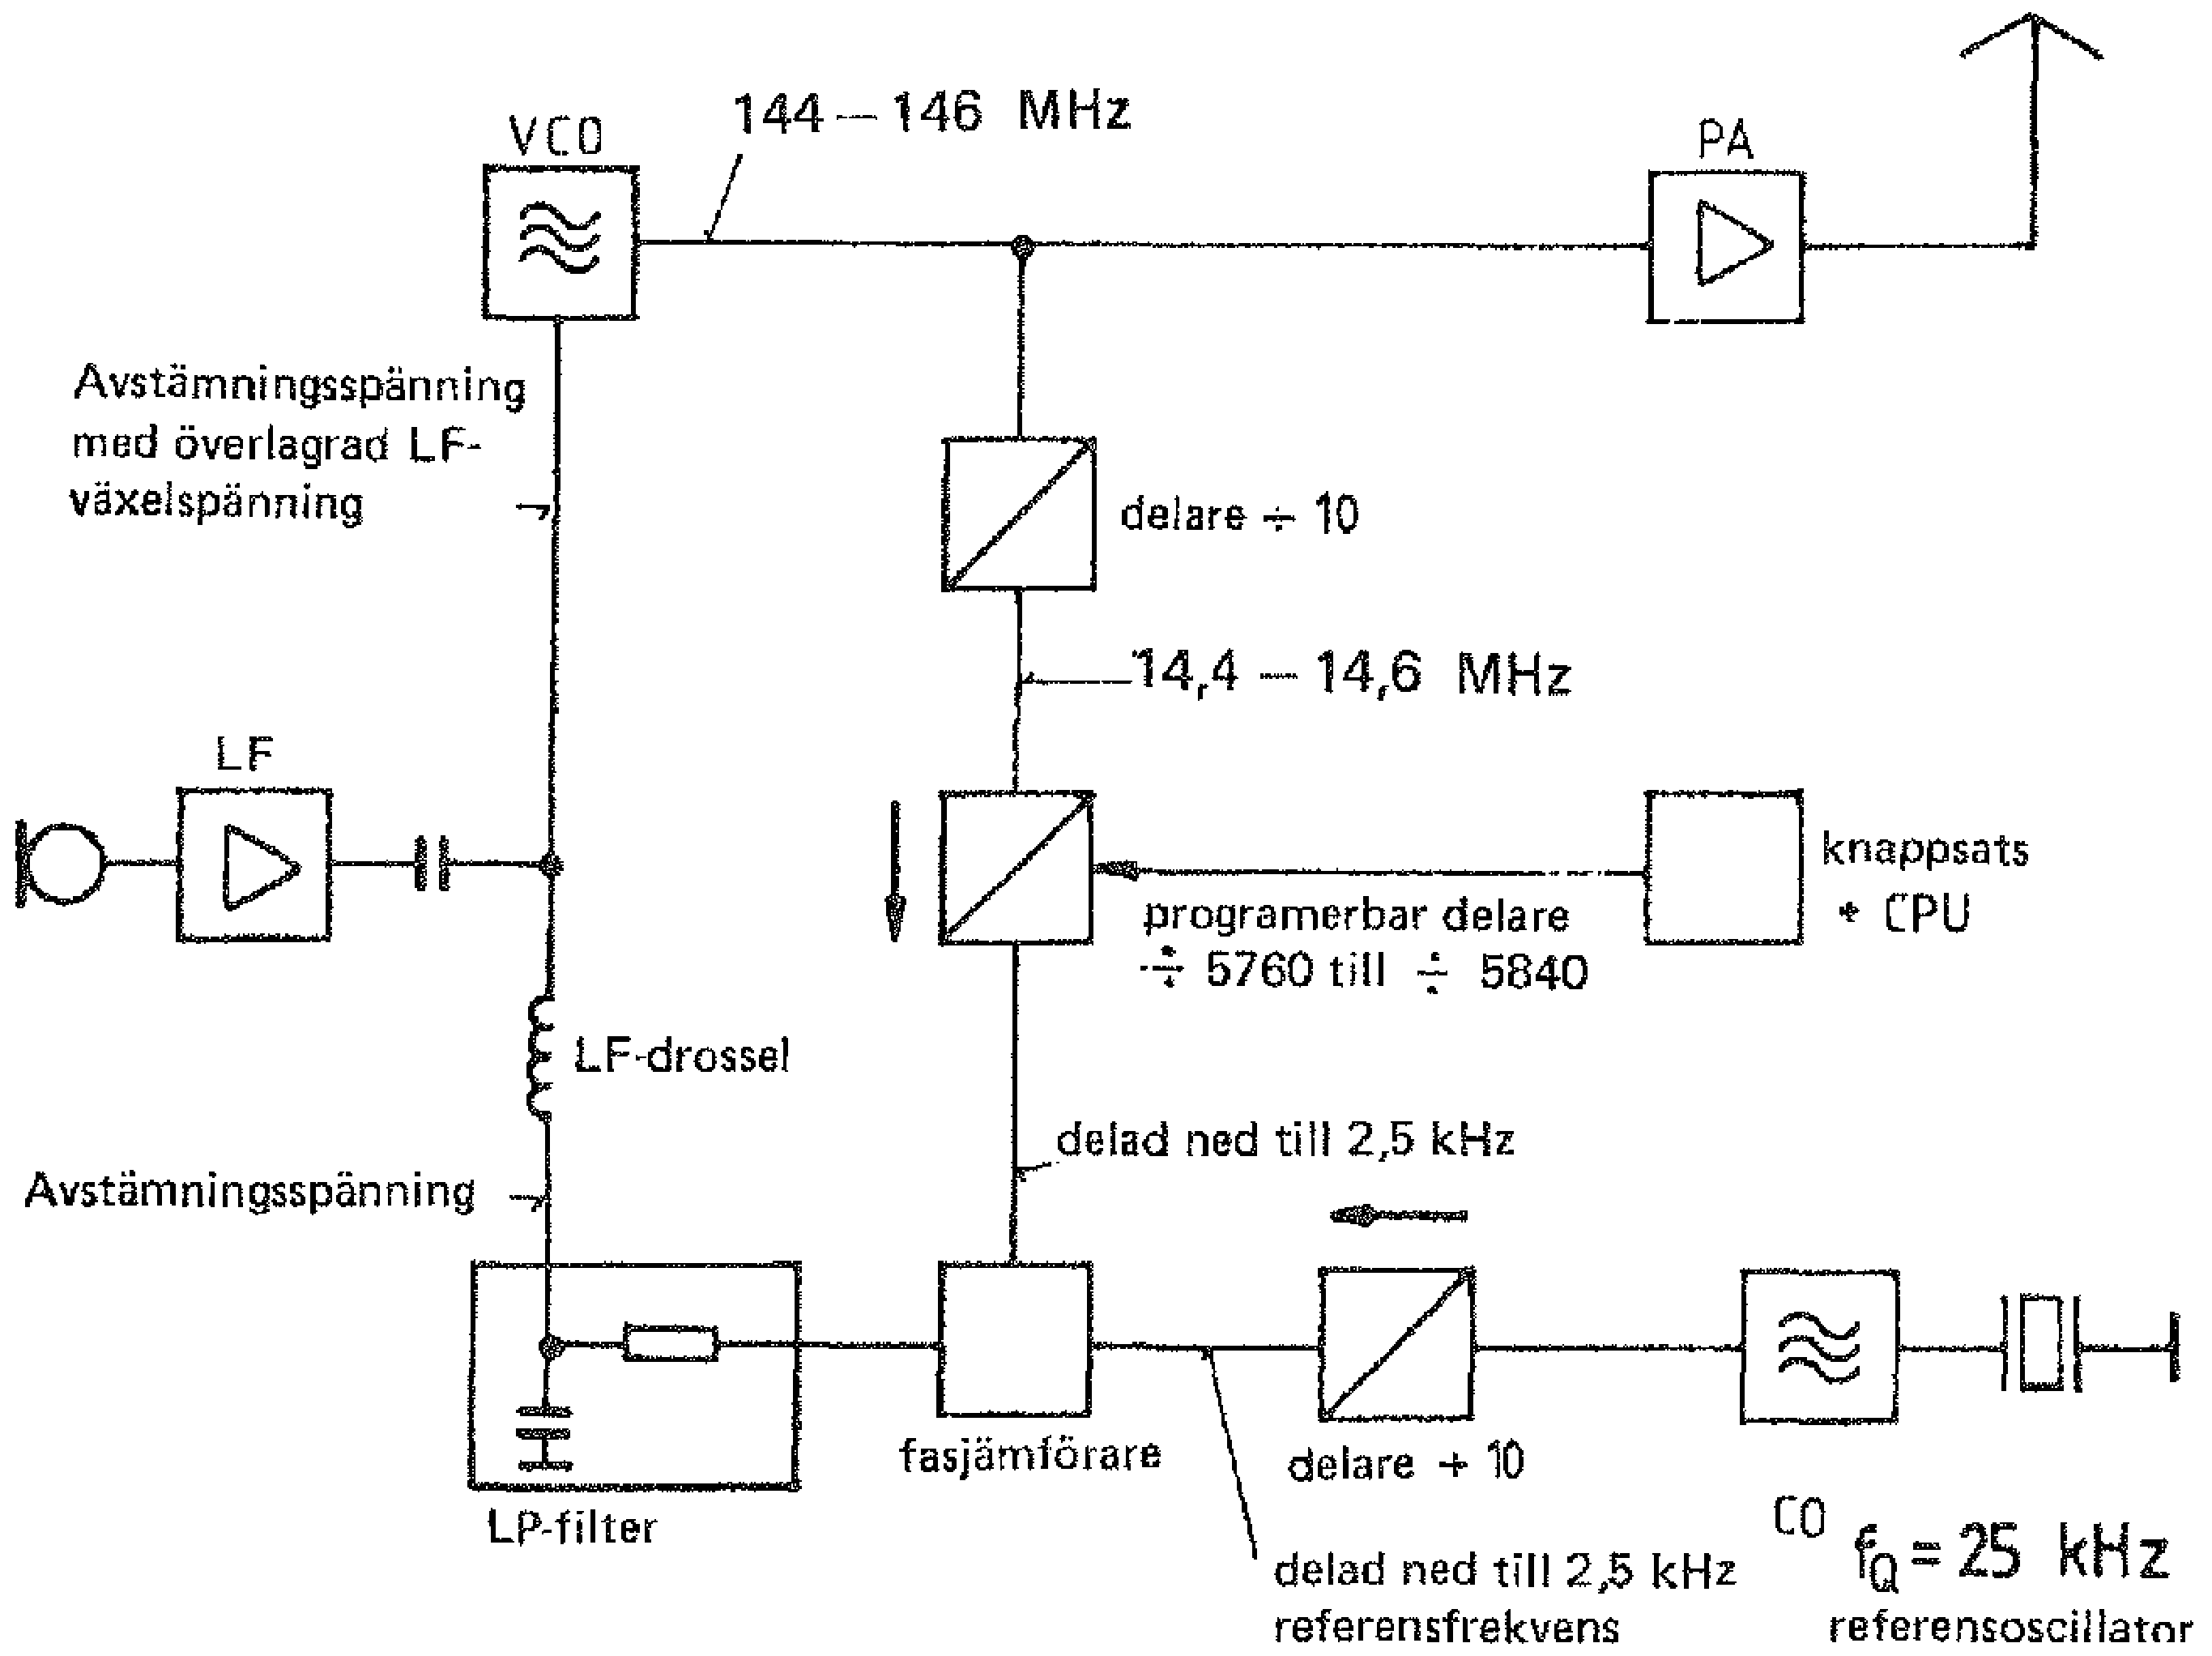
\includegraphics[width=\textwidth]{images/cropped_pdfs/bild_2_5-07.pdf}
  \caption{PLL-styrd FM-sändare för FM}
  \label{fig:bildII5-7}
\end{figure}

Bild \ref{fig:bildII5-7} visar en PLL-styrd rak sändare med en
VCO (spänningsstyrd oscillator) och ett PA (effektförstärkare).

VCO ingår som det frekvensstyrda elementet i en PLL.
Utfrekvensen från VCO (ärvärdet) avläses och delas periodiskt med talet 10
och matas in i en programmerbar frekvensdelare.
Eftersom frekvensområdet för VCO är 144--146~MHz, kommer infrekvensen till
den programmerbara delaren att ligga i området 14,4--14,6~MHz.
Delningstalet i denna delare kan programmeras in i steg om 1 mellan
talen 5760 och 5840.

Med den första delarens divisor 10 och den andra delarens divisor
inställd t.ex. på 5760, så avges ur delarkedjan en puls varje gång som
VCO har genomfört 57600 svängningar.
Vid en VCO-frekvens av 144~MHz (144000~kHz) motsvaras divisorn
57600 (= \(10 \cdot 5760\)) av en pulsfrekvens av 2,5~kHz ut från räknarkedjan.
På samma sätt kommer en VCO-frekvens av 144025~kHz och divisorn
57610 (= \(10 \cdot 5761\)) också att ge en pulsfrekvens av 2,5~kHz,
likaså 146~MHz och divisorn 58400 o.s.v.

VCO-frekvensen låses alltså i intervall om 25~kHz till närmaste
delningstal, för att uppnå en pulsfrekvens av 2,5~kHz.
Om VCO-frekvensen (är-värdet) avviker från det inställda delningstalet
(bör-värdet), så kommer pulsfrekvensen att bli högre eller lägre än
2,5~kHz.

Pulsfrekvensen jämförs i en s.k. fasjämförare med en kristallstyrd
referensfrekvens som efter en delning med 10 också är 2,5~kHz.
Utspänningen från jämföraren är en likspänning, som intar ett
medelvärde då infrekvenserna är lika, men ett högre eller lägre värde
när de skiljer.
Denna likspänning används för att kontinuerlig styra VCO-frekvensen
till likhet med börvärdet.
Regleringsförloppets hastighet bestäms av tidskonstanten i ett
lågpassfilter, det s.k. loop-filtret.

Sändningsfrekvensen regleras alltså med styrspänningen.
Med samma spänning går det också att frekvensmodulera oscillatorn.
Det görs så, att LF-signalen från modulatorn överlagras på styrspänningen genom
additiv blandning (se kapitel \ref{blandare}) via en kondensator.
De variationer i reglerspänningen som kommer av talet är snabbare än
loopfiltrets tidskonstant.
Variationerna av talet hinner därför inte uppfattas som frekvensavvikelser och
blir därför inte utreglerade.
Drosseln efter loop-filtret förhindrar att moduleringssignalen
kortsluts av filtrets kondensator.

Frekvensinställningen, d.v.s. programmeringen av delaren kan utföras
på flera sätt. Exempel på inställningsorgan är tumhjuls-omkopplare,
logikkretsar i kombination med en knappsats o.s.v.

\subsubsection{PLL-styrd sändare för kortvåg}

\begin{figure}
  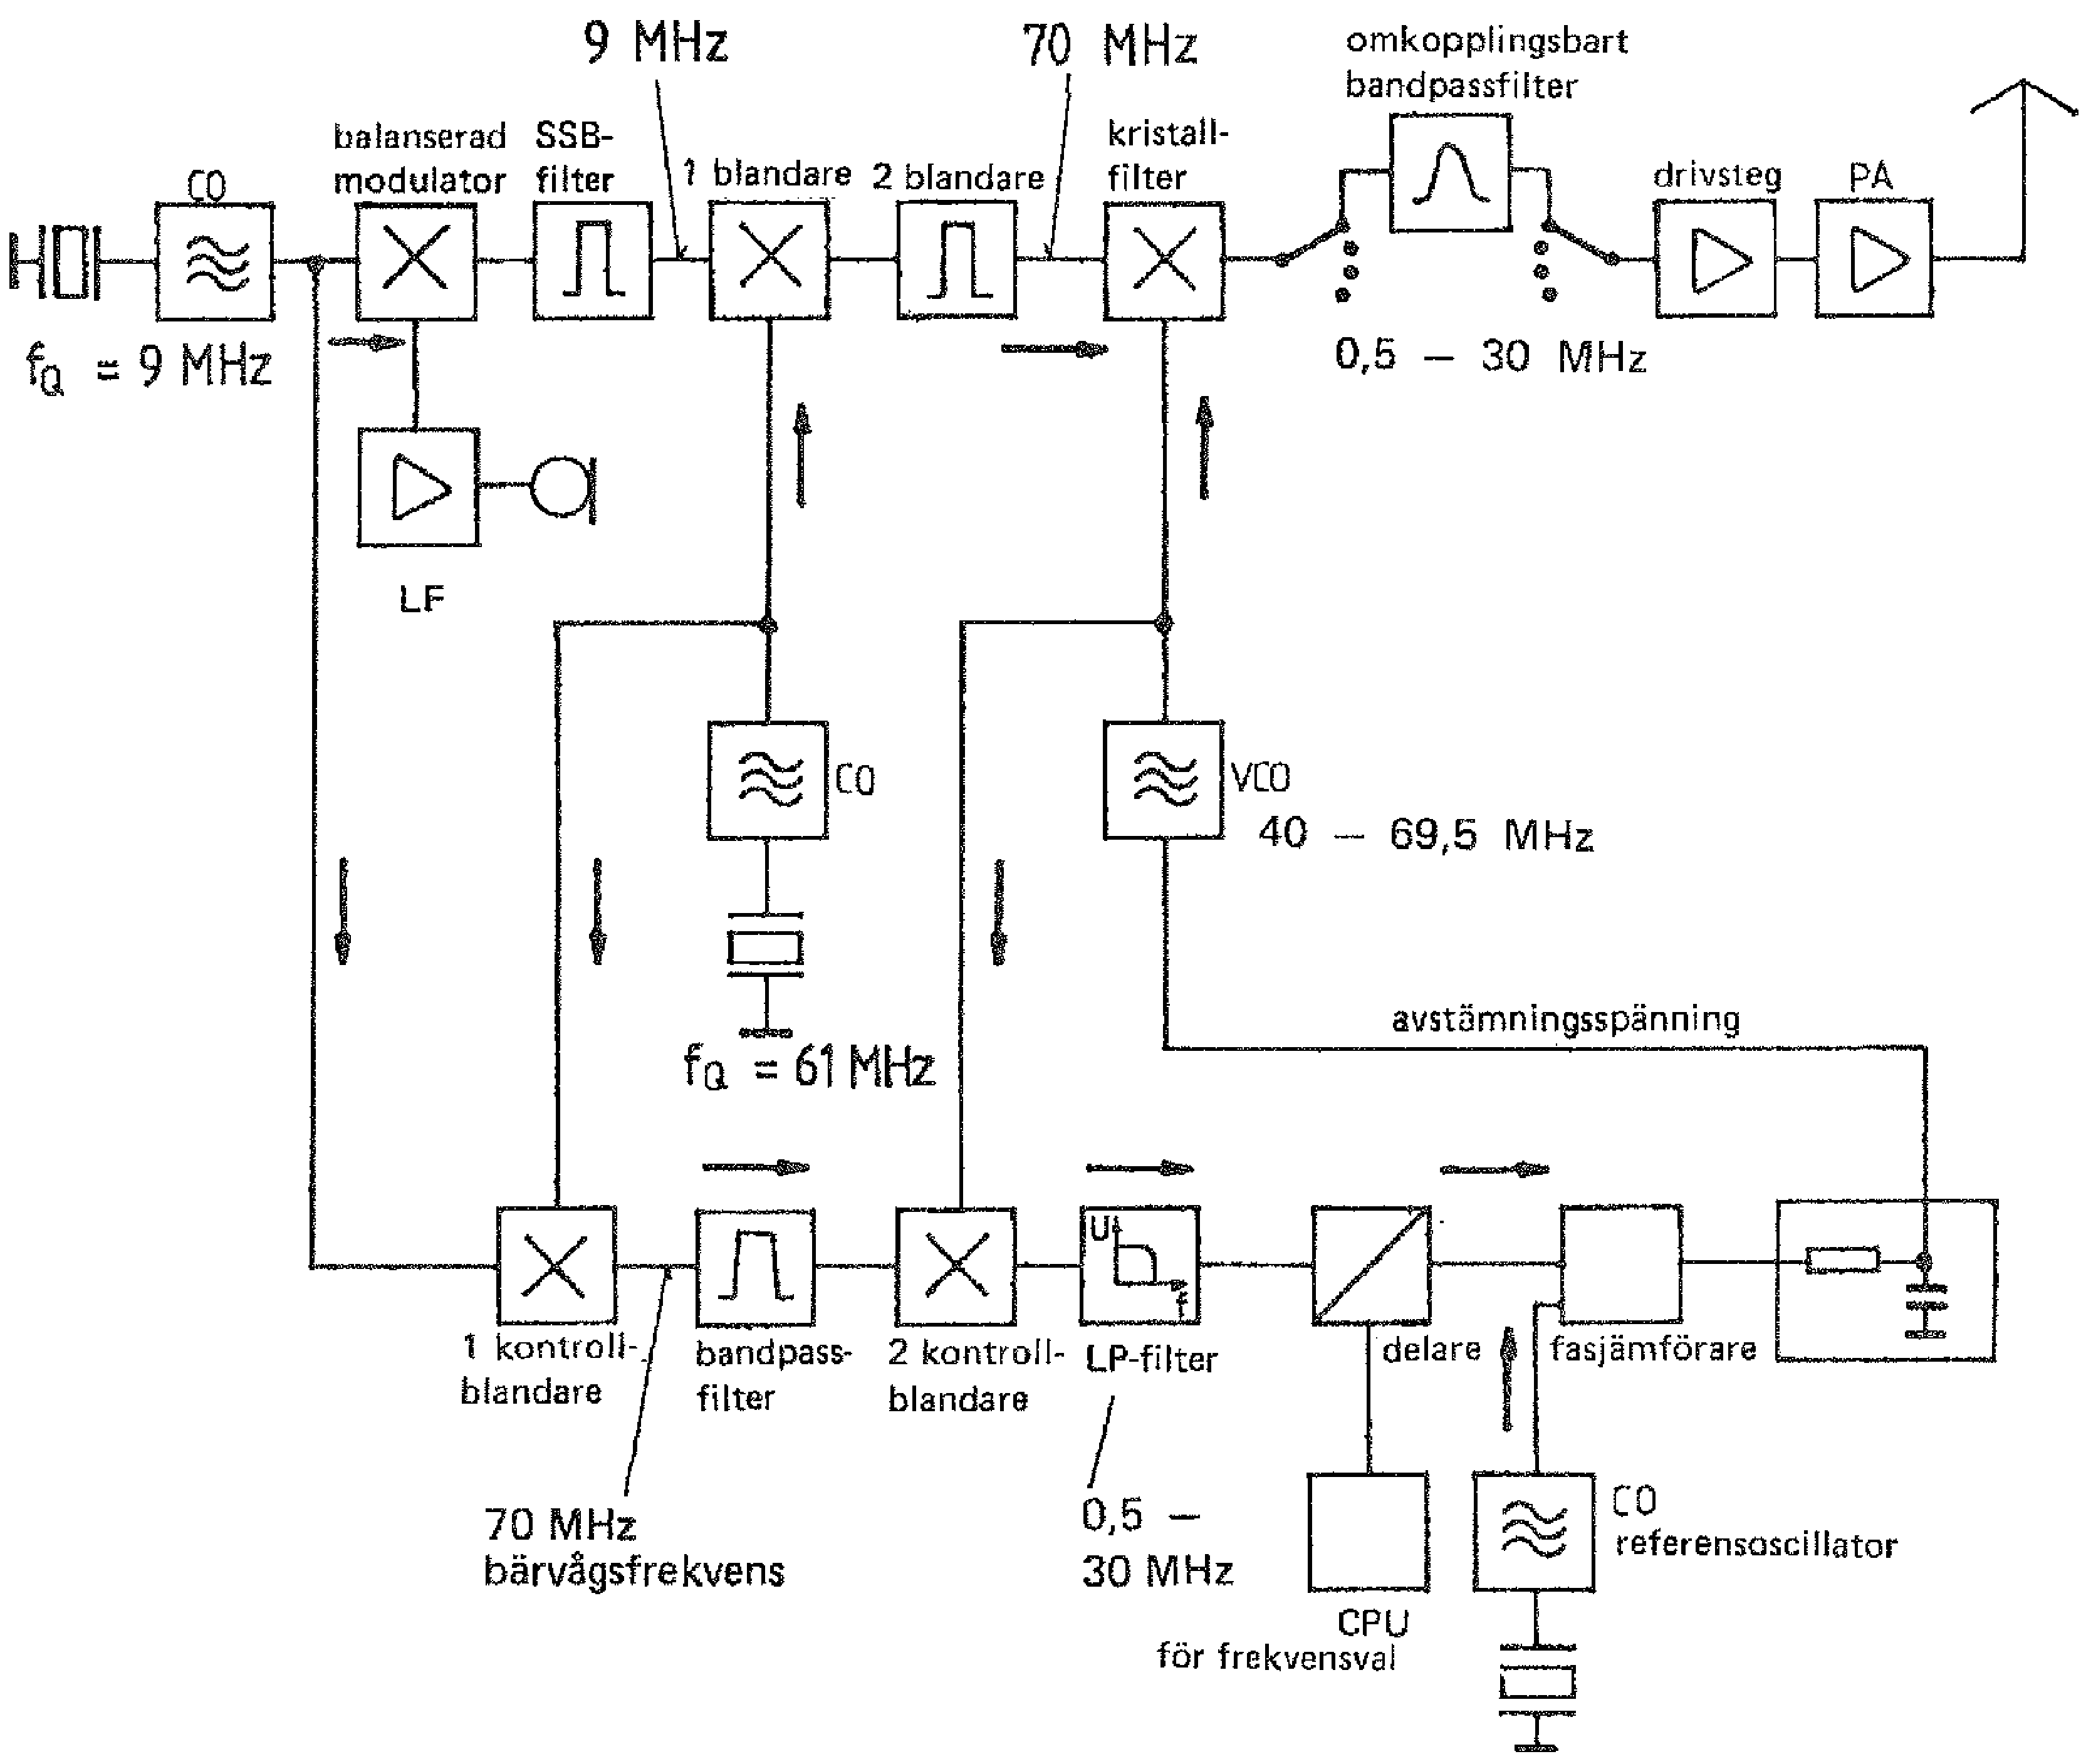
\includegraphics[width=\textwidth]{images/cropped_pdfs/bild_2_5-08.pdf}
  \caption{PLL-styrd SSB-sändare för kortvåg}
  \label{fig:bildII5-8}
\end{figure}

Bild \ref{fig:bildII5-8} visar ett avancerat koncept för en kortvågssändare.
SSB-signalen alstras på frekvensen 9~MHz och blandas med 61~MHz i 1:a
blandaren.

Summafrekvensen 70~MHz filtreras fram som mellanfrekvens.
Den önskade sändningsfrekvensen fås genom att blanda 70~MHz MF med
frekvensen från VCO och därefter filtrera fram skillnadsfrekvensen.
VCO i detta exempel täcker frekvensområdet 40--69,5~MHz.
Således blir sändarens täckningsområde 1,5--30~MHz.
För att filterfunktionen ska bli optimal, kan den delas upp på flera
valbara filtersektioner, t.ex. ett per amatörband.
Valet kan ske automatiskt och styrt av frekvensläget på VCO.

Den absoluta ändringen mellan de två extrema sändningsfrekvenserna är
så stor som 28,5~MHz eller 1:20.
Frekvensändringen i VCO är 29,5~MHz, men där är ändringsförhållandet
mellan de extrema frekvenserna endast 1:1,74, vilket kan täckas av en enda VCO.
Vid en lägre 2:a MF-frekvens skulle det behövas flera omkopplingsbara
VCO för att täcka hela frekvensområdet

\textbf{Exempel:} Vid en MF på 9~MHz behöver VCO-funktionen täcka 9,5--39~MHz,
d.v.s. 1:4,11, vilket är för mycket för en VCO.

SSB-signalen efter 2:a blandaren är inte lämplig att använda i
regleringsslingan i PLL.
Anledningen är att bärvågen är undertryckt i denna signal och att därför
HF-frekvenserna i det resterande sidbandet varierar i takt med de
modulerande LF-frekvenserna.

I konceptet på bilden rekonstrueras bärvågen i en 1:a kontrollblandare,
genom blandning av de två CO-frekvenserna 9 och 61~MHz.
Den framfiltrerade bärvågen med frekvensen 70~MHz blandas med
VCO-frekvensen i 2:a kontrollblandare och ur denna signal
framfiltreras den rekonstruerade bärvågen.
Denna stämmer perfekt med den undertryckta bärvågens frekvens och
innehåller inga LF-signaler.
Bärvågsfrekvensen delas i en programmerbar frekvensdelare och jämförs
med frekvensen från en kristallstyrd referensoscillator CO.
Ur fasjämföraren erhålls en likspänning som styr VCO via ett loop-filter.
Frekvensen ställs in genom att programmera delaren i PLL.

I en modern sändare finns ofta en mikroprocessor, som erbjuder talrika
möjligheter bl.a. till frekvensinställning, minnen och avsökning av
frekvenser.

Det beskrivna konceptet är avancerat.
Frekvensen i alla oscillatorer styrs av samma referensoscillator.
Frekvensstabiliteten beror alltså enbart på referensoscillatorns stabilitet.

Omkopplingen mellan LSB och USB kan göras antingen genom att behålla
SSB-filtret och ändra frekvensen 9~MHz med ett värde så att filtret
blir verksamt i det motsatta sidbandet eller genom att behålla
frekvensen 9~MHz och byta till ett SSB-filter som är verksamt i det
motsatta sidbandet.

En PLL-styrd sändare har både kristalloscillatorns stabilitet och variabel
frekvens över ett stort frekvensområde trots ett litet antal styrkristaller.
En sådan sändare kan relativt enkelt styras digitalt.

En principiell nackdel med alla sändare med PLL-oscillator är fasbruset.
En annan nackdel är den stora komponentmängden
(se kapitel \ref{superheterojämförelse}).

\section{Egenskaper i sändare}
\textbf{HAREC
  a.\ref{HAREC.a.5.4}\label{myHAREC.a.5.4}
}

Sändare har många olika egenskaper som man ska vara uppmärksam på, dels för
att ha en effektiv sändare, dels för att få bra kvalitet på sändning och dels
för att inte störa grannkanaler eller på andra band.

\subsection{Frekvensstabilitet}
\textbf{HAREC
  a.\ref{HAREC.a.5.4.1}\label{myHAREC.a.5.4.1}
}
\index{frekvensstabilitet}

\emph{Frekvensstabiliteten} (eng. \emph{frequency stability}) är en
grundläggande egenskap, eftersom en sändare som inte är frekvensstabil nog
kommer bli svår för en mottagare att följa och uppfatta.
Dessutom riskerar man att störa grannkanaler.
Mindre avdrift i frekvens kan tolereras, men helst ska den uppfattas som
helt stabil.

I gamla tider så var resonatorerna LC-kretsar, och både mekanik och elektronik
kunde driva betänkligt.
Med modernare kristallstyrda sändare, där man använder PLL eller DDS
synteser så kan frekvensstabiliteten härledas till en enskild
kristalloscillator.
Denna är typiskt en okompenserad kristall, med man brukar kunna välja en
temperatur-kompenserad kristalloscillator -- TCXO eller en ugnskompenserad
kristalloscillator -- OCXO.
Det kan även förekomma att man kan låsa på en extern referensfrekvens,
ofta 10~MHz.

\subsection{RF-bandbredd}
\textbf{HAREC
  a.\ref{HAREC.a.5.4.2}\label{myHAREC.a.5.4.2}
}
\index{RF bandbredd}
\index{splatter}
\index{spegelfrekvenser}

\emph{RF bandbredden} (eng. \emph{RF bandwidth}) är den bandbredd som den
modulerade signalen har när den kommer ut ur sändaren.
Det är viktigt att den är begränsad så att den håller sig inom de gränser
som finns för signaltypen, så att sändaren inte stör grann-kanalerna.
T.ex. kan en sändare anpassad för FM 25~kHz kanaldelning modulera för starkt för
NFM 12,5~kHz kanaldelning och helt enkelt störa grann-kanalerna.

Det är ofta svårt att begränsa RF-bandbredden direkt på utgången av sändaren,
eftersom den förväntas kunna byta kanal.
Istället så begränsar man bandbredden på mellanfrekvens direkt vid modulatorn,
och innan frekvens-skiftningen upp till rätt frekvens.
Detta kräver dock att efterföljande steg är linjära nog att inte skapa oönskade
sidband i så kallat splatter eller tar upp spegelfrekvenser.

\subsection{Sidband}
\textbf{HAREC
  a.\ref{HAREC.a.5.4.3}\label{myHAREC.a.5.4.3}
}
\index{sidband}
\index{övre sidband}
\index{sidband!övre}
\index{Upper Side Band (USB)}
\index{USB}
\index{undre sidband}
\index{sidband!undre}
\index{Lower Side Band (LSB)}
\index{LSB}

När man sänder skapas \emph{sidband} (eng. \emph{side band}).
För AM och SSB så skapas bägge, \emph{övre sidbandet}
(eng. \emph{Upper Side Band (USB)}) eller \emph{undre sidbandet}
(eng. \emph{Lower Side Band (LSB)}) av den modulerade signalen.
För SSB undertrycks även bärvågen.
För FM skapas bredare sidband som behöver filtreras.

\subsection{Ljudbandbredd}
\textbf{HAREC
  a.\ref{HAREC.a.5.4.4}\label{myHAREC.a.5.4.4}
}
\index{ljudbandbredd}
\index{audio bandwidth}

Bandbredden på ljudsignalen, den så kallade \emph{ljudbandbredden} (eng.
\emph{audio bandwidth}) in kan vara väldigt stor, och det är därför viktigt
att sändaren begränsar den bandbredden så att sändaren inte råkar modulera
utanför sin kanal, något som främst påverkar bandbredds begränsning uppåt,
oftast 3~kHz för amatörradio.
Bandbredden kan också behöva begränsas nedåt vid 300~Hz för att inte råka
störa t.ex signalering med subtoner.
Denna nedre begränsning kan dock ibland behöva sättas ur spel för att
kunna skicka ut subtonssignaler, men även för andra former av signaler.

\subsection{Olinjaritet}
\textbf{HAREC
  a.\ref{HAREC.a.5.4.5}\label{myHAREC.a.5.4.5}
}
\index{olinjaritet}
\index{nonlinearity}
\index{splatter}

\emph{Olinjaritet} (eng. \emph{nonlinearity}) i ett sändarsteg ger dels
övertoner som behöver begränsas, ofta genom ett filter på utgången, men man
försöker även begränsa hur olinjärt steget tillåts bli.
För tal kommer olinjäritet även att påverka intermodulationen mellan flera
olika frekvenser i tal, vilket dels skapar störningar inom bandet men även
utanför och därmed breddar det.
Detta kallas för splatter och är en oönskad egenskap.
God linjäritet även vid höga effekter är därför eftersträvansvärt.
Ibland kan man ha så mycket olinjäritet att taltydligheten blir låg, det
kan därför vara lämpligt att dra ned något på effekten så taltydligheten går
upp, vilket då ger bättre signalrapport än när intermodulationen är för hög.

\subsection{Utgångsimpedans}
\textbf{HAREC
  a.\ref{HAREC.a.5.4.6}\label{myHAREC.a.5.4.6}
}
\index{utgångsimpedans}

\emph{Utgångsimpedansen} (eng. \emph{output impedance}) är förstärkarens
drivegenskaper och de ska oftast vara anpassade till kabel.
Oftast är det 50~ohm, men för förstärkare som har inbyggd matchbox,
automatisk eller ej, så kan förstärkarens utimpedans anpassas
för att kunna driva en antennsystem med större avvikelser i impedans.
En god matchning i impedans krävs för att få en bra energiöverföring av den
tillförda energin utan att för mycket studsar tillbaka.
Många sändare har skyddskretsar som drar ned uteffekten vid för stor
reflekterad energi, för att skydda slutsteget, och det gör att ett
impedansmatchfel ger ännu större reduktion i utsänd effekt än vad själva
impedansfelet i sig skulle motivera.

\subsection{Uteffekt}
\textbf{HAREC
  a.\ref{HAREC.a.5.4.7}\label{myHAREC.a.5.4.7}
}
\index{uteffekt}

\emph{Uteffekten} (eng. \emph{output power}) är den effekt som sändaren är
kapabel att sända, på ett visst band, vid god utgångsmatchning.
Ofta är den mätt i p.e.p. för att matcha kraven från övervakande myndigheter.
Det kan gå att få högre faktisk effekt ur en sändare, men då kommer den vara
så pass olinjär att den inte förväntas klara krav på splatter.

\subsection{Effektivitet}
\textbf{HAREC
  a.\ref{HAREC.a.5.4.8}\label{myHAREC.a.5.4.8}
}
\index{effektivitet}

\emph{Effektiviteten} (eng. \emph{efficiency}) på en sändare eller slutsteg
är den utsända effekten i förhållande till den tillförda effekten.
Effektiviteten varierar med uteffekt och frekvens.

\subsection{Frekvensdeviation}
\textbf{HAREC
  a.\ref{HAREC.a.5.4.9}\label{myHAREC.a.5.4.9}
}
\index{frekvensdeviation}

\emph{Frekvensdeviationen} är den maximala avvikelsen från bärvågen som
tillåts vid frekvensmodulation.

\subsection{Modulationsindex}
\textbf{HAREC
  a.\ref{HAREC.a.5.4.10}\label{myHAREC.a.5.4.10}
}
\index{modulationsindex}
\index{modulationsdjup}

\emph{Modulationsindex} (eng. \emph{modulation index}), eller även
\emph{modulationsdjupet}, anger hur djup modulation av bärvågen är.
För hög modulations undertrycker bärvågen och kan göra det svårt för
mottagaren att detektera.
För låg modulation ger svaga sidband att förmedla tal, och för mycket
av energin går till att sända enbart bärvåg.

\subsection{CW klickar}
\textbf{HAREC
  a.\ref{HAREC.a.5.4.11}\label{myHAREC.a.5.4.11}
}

Vid CW kan för snabb stig och falltid på bärvågen ge onödig bandbredd och
uppfattas som klickar eller chirpar. Då detta är störande ska bandbredden
begränsas genom att filtrera bärvågens till- och frånslag.

\subsection{SSB övermodulation och splatter}
\textbf{HAREC
  a.\ref{HAREC.a.5.4.12}\label{myHAREC.a.5.4.12}
}
\index{övermodulation}
\index{SSB!övermodulation}
\index{splatter}

Övermodulation vid SSB ger intermodulation och splatter, vilket ger dels en
signal om är svår att läsa och dels en för bred signal.

\subsection{RF spurioser}
\textbf{HAREC
  a.\ref{HAREC.a.5.4.13}\label{myHAREC.a.5.4.13}
}

Utöver den förväntade bärvågen kan en sändare skicka ut frekvenser som vare
sig tillhör bärvåg och dess sidband. Harmoniska undertoner samt helt andra
orelaterade frekvenser ska vara undertryckta.
Detta regleras i EMC standarden för radioutrustning, i det här fallet för
amatörradio.

\subsection{Chassistrålning}
\textbf{HAREC
  a.\ref{HAREC.a.5.4.14}\label{myHAREC.a.5.4.14}
}

En sändare förväntas kunna leverera en stor effekt ut på antennutgången, men
från själva inneslutningen, chassit, och övriga anslutningar ska sändaren
inte sända bärvåg, sidband eller några andra signaler.

\subsection{Fasbrus}
\textbf{HAREC
  a.\ref{HAREC.a.5.4.15}\label{myHAREC.a.5.4.15}
}
\index{fasbrus}

\emph{Fasbrus} (eng. \emph{phase noise}) är en egenskap hos alla oscillatorer,
som ger en fasmodulation av bärvågen.
Alla steg i en sändare bidrar med brus och ger sammanlagt det totala fasbruset.
En sändares fasbrus kan sträcka sig långt utanför den normala modulerade
bandbredden, och speciellt för repeatrar så kan sändarens fasbrus höja
brusgolvet för mottagaren om inte korrekt trimmade duplexfilter
används för att undertrycka sändarens fasbrus på mottagarens ingångsfrekvens.
